%%%%%%%%%%%%%%%%%%%%%%%%%%%%%%%%%%%%%%%%%%%%%%%%%%%%%%%%%%%%%%%%%%%%%%%%%%%%%%%%%%%%%%%%%%%%%%%%
%
% CS484 Written Question Template
%
% Acknowledgements:
% The original code is written by Prof. James Tompkin (james_tompkin@brown.edu).
% The second version is revised by Prof. Min H. Kim (minhkim@kaist.ac.kr).
%
% This is a LaTeX document. LaTeX is a markup language for producing 
% documents. Your task is to fill out this document, then to compile 
% it into a PDF document. 
%
% 
% TO COMPILE:
% > pdflatex thisfile.tex
%
% If you do not have LaTeX and need a LaTeX distribution:
% - Personal laptops (all common OS): www.latex-project.org/get/
% - We recommend latex compiler miktex (https://miktex.org/) for windows,
%   macTex (http://www.tug.org/mactex/) for macOS users.
%   And TeXstudio(http://www.texstudio.org/) for latex editor.
%   You should install both compiler and editor for editing latex.
%   The another option is Overleaf (https://www.overleaf.com/) which is 
%   an online latex editor.
%
% If you need help with LaTeX, please come to office hours. 
% Or, there is plenty of help online:
% https://en.wikibooks.org/wiki/LaTeX
%
% Good luck!
% Min and the CS484 staff
%
%%%%%%%%%%%%%%%%%%%%%%%%%%%%%%%%%%%%%%%%%%%%%%%%%%%%%%%%%%%%%%%%%%%%%%%%%%%%%%%%%%%%%%%%%%%%%%%%
%
% How to include two graphics on the same line:
% 
% \includegraphics[width=0.49\linewidth]{yourgraphic1.png}
% \includegraphics[width=0.49\linewidth]{yourgraphic2.png}
%
% How to include equations:
%
% \begin{equation}
% y = mx+c
% \end{equation}
% 
%%%%%%%%%%%%%%%%%%%%%%%%%%%%%%%%%%%%%%%%%%%%%%%%%%%%%%%%%%%%%%%%%%%%%%%%%%%%%%%%%%%%%%%%%%%%%%%%

\documentclass[11pt]{article}

\usepackage[english]{babel}
\usepackage[utf8]{inputenc}
\usepackage[colorlinks = true,
            linkcolor = blue,
            urlcolor  = blue]{hyperref}
\usepackage[a4paper,margin=1.5in]{geometry}
\usepackage{stackengine,graphicx}
\usepackage{fancyhdr}
\setlength{\headheight}{15pt}
\usepackage{microtype}
\usepackage{times}
\usepackage{booktabs}
\usepackage{gensymb}
\usepackage{commath}

% From https://ctan.org/pkg/matlab-prettifier
\usepackage[numbered,framed]{matlab-prettifier}

\frenchspacing
\setlength{\parindent}{0cm} % Default is 15pt.
\setlength{\parskip}{0.3cm plus1mm minus1mm}

\pagestyle{fancy}
\fancyhf{}
\lhead{Project Writeup}
\rhead{CS 484}
\rfoot{\thepage}

\date{}

\title{\vspace{-1cm}Homework 4 Writeup}


\begin{document}
\maketitle
\vspace{-3cm}
\thispagestyle{fancy}

\section*{Instructions}
\begin{itemize}
  \item Describe any interesting decisions you made to write your algorithm.
  \item Show and discuss the results of your algorithm.
  \item Feel free to include code snippets, images, and equations.
  \item Use as many pages as you need, but err on the short side If you feel you only need to write a short amount to meet the brief, th
  
  \item \textbf{Please make this document anonymous.}
\end{itemize}

\section*{Algorithm Implementation}

Algorithms of this project is implemented in three parts. 

\subsection{Interest Point Detection}
The interest points of a pair of images is found using Harris corner detector. Full code is shown below. In line 7, a Gaussian filter is created. The gradient of the filter is calculated in lines 9-14. They are then convolbed with the image to find the image gradients. The gradient of the filter is calculated instead of that of the image to reduced the effects of noise in the image. It is still the same operation as finding the gradient of the blurred image directly. In lines 20-22, image gradients are convolved with the Gaussian filter to find the second moment matrix \emph{M}. In line 24, the cornerness is calculated using the formula $C=det(M)-\alpha trace(M)^2$. In line 26, the indices of pixels at which the cornerness is less than a threshold is returned.

\begin{lstlisting}[style=Matlab-editor]
function [x, y, confidence, scale, orientation] = get_interest_points(image, descriptor_window_image_width)

alpha = 0.05;
threshold = -0.011;

%apply double derivative to the filter first then apply to the image, to remove the effects of noise
gauss_filter = fspecial('Gaussian', 11, 1);

Dx = imderivative(gauss_filter, [1 0]);
Dy = imderivative(gauss_filter, [0 1]);
Dxy = imderivative(gauss_filter, [1 1]);

Dx2 = Dx.*Dx;
Dy2 = Dy.*Dy;

Ix2 = imfilter(image, Dx2, 'symmetric', 'same', 'conv');
Iy2 = imfilter(image, Dy2, 'symmetric', 'same', 'conv');
Ixy = imfilter(image, Dxy, 'symmetric', 'same', 'conv');

Gx2 = imfilter(Ix2, gauss_filter, 'symmetric', 'same', 'conv');
Gy2 = imfilter(Iy2, gauss_filter, 'symmetric', 'same', 'conv');
Gxy = imfilter(Ixy, gauss_filter, 'symmetric', 'same', 'conv');

C = Gx2.*Gy2-(Gxy.*Gxy)-alpha*((Gx2+Gy2).*(Gx2+Gy2));

[y,x] = find(C<threshold);

end

function I = imderivative(img,direction)
It = imtranslate(img,-direction,'OutputView','full');
Ip = padarray(img,flip(direction),0,'pre');
I = It-Ip;
I = I(1:size(I,1)-direction(2),1:size(I,2)-direction(1));
end
\end{lstlisting}

\subsection{Descriptor Calculation}
Desriptors at each interest point is calculated into a $4*4*8=128$ dimension feature. Code is shown below. In lines 3-10, blurred image gradients are calculated by convolving the gradients of a Gaussian filter to the image. Then for each interest point, a patch of image of size $16*16$ in $x$ and $y$ gradients is found in lines 16 and 17. The orientation at each of the 16 pixels is calculated in line 19 and mapped to range [$0\degree, 360\degree$]. The result is divided by $45\degree$ to convert to bin index. For each of the 16 $4*4$ patches inside the $16*16$, the number of pixels at each bin slot is calculated in line 25. It was concatenated at the i'th feature at $features(i)$ in line 26. For each of the $1*128$ feature, it was normalized by dividing it by the maximum element in lines 30-31. The final array of features was raised to a power of $0.8$ following the trick provided in the comment of the \emph{get\_descriptors.m} file at the top.

\begin{lstlisting}[style=Matlab-editor]
function [features] = get_features(image, x, y, descriptor_window_image_width)

features = zeros(size(x,1), 128, 'single');
gauss_filter = fspecial('Gaussian', 4, 0.6);

Dx = imderivative(gauss_filter, [1 0]);
Dy = imderivative(gauss_filter, [0 1]);

Ix = imfilter(image, Dx, 'symmetric', 'same', 'conv');
Iy = imfilter(image, Dy, 'symmetric', 'same', 'conv');
for i = 1:size(x,1)
    if(x(i)<8 || y(i)<8 || x(i)+8>size(Ix,2) || y(i)+8>size(Iy,1))
        % skip out of image patches
        continue
    end
    patch_Ix = Ix((y(i)-7):(y(i)+8),(x(i)-7):(x(i)+8));
    patch_Iy = Iy((y(i)-7):(y(i)+8),(x(i)-7):(x(i)+8));
    %computing the tangent in degrees
    orientation = radtodeg(atan2(patch_Iy,patch_Ix))+180;
    %computing the 8 quandrants
    quads = ceil(orientation/45);
    for m = 1:4
        for n = 1:4
            patch4 = quads(m*4-3:m*4, n*4-3:n*4);
            qcounts = histcounts(patch4,0.5:1:8.5);
            features(i,(4*(m-1)+(n-1))*8+1:(4*(m-1)+(n-1))*8+8) = qcounts;
        end
    end
    %normalize each feature
    [mf,~] = max(features(i,:));
    features(i,:) = features(i,:)/mf;
end
features = features.^0.8;
end
\end{lstlisting}
\subsection{Feature Matching}
Features calculated from a pair of images by \emph{get\_descriptors.m} is matched using the \emph{NNDR} method. Code is shown below. To match features, distance from every feature in one image to every feature in another image should be calculated, called the pairwise distance. The pairwise distance between the two feature arrays was calculated using a custom function called \emph{pairwise\_distance} in lines 31-39. Internally, the norm function of MATLAB  was used to calculate sidtance. Such distances were sorted in ascending order to move close features to the front. The \emph{NNDR} value is calculated using the formula $\frac{\norm{D_A -D_B}}{\norm{D_A - D_C}}$ in line 6. The matched indices are filled in lines 8-11 using the sorted index. In line 13, the good indices are defined as indices at which \emph{NNDR} is less than a threshold. The confidence value was calculated by the element-wise inverse because a low \emph{NNDR} means a confident match. Then the confidence and matches are sorted and taken only the top 100 because the top 100 is the minimum requirement for grading.

\begin{lstlisting}[style=Matlab-editor]
function [matches, confidences] = match_features(features1, features2)

num_features = min(size(features1, 1), size(features2,1));
pd = pairwise_distance(features1, features2);
[sortdist, sortindex] = sort(pd,2,'ascend');
nndr = sortdist(:,1)./sortdist(:,2);

matches = zeros(size(features1, 1), 2);

matches(:,1) = 1:size(features1);
matches(:,2) = sortindex(:,1);

good_indices = find(nndr<0.93);

matches = matches(good_indices,:); 

confidences = 1./nndr(good_indices);

[confidences, ind] = sort(confidences, 'descend');

% get top 100 indices
confidences = confidences(1:min(100,size(confidences)));
ind = ind(1:min(100,size(matches)));
matches = matches(ind,:);

end

function pd = pairwise_distance(X,Y)
    pd = zeros(size(X,1),size(Y,1));
    for m=1:size(X,1)
        for n=1:size(Y,1)
            %sum of squares of elements
            pd(m,n) = norm(X(m,:)-Y(n,:));
        end
    end
end
\end{lstlisting}

\section*{Results}

The interest points are matched in Notre Dame, Mount Rushmore, and Episcopal Gaudi images in Figures~\ref{fig:nd}, ~\ref{fig:mr} and ~\ref{fig:eg}, respectively. Because scale and orientation invariance of feature matching is not implemented, accuracy in Mount Rushmore and Episcopal Gaudi images are not high.

\begin{figure}[h!]
	\centering
	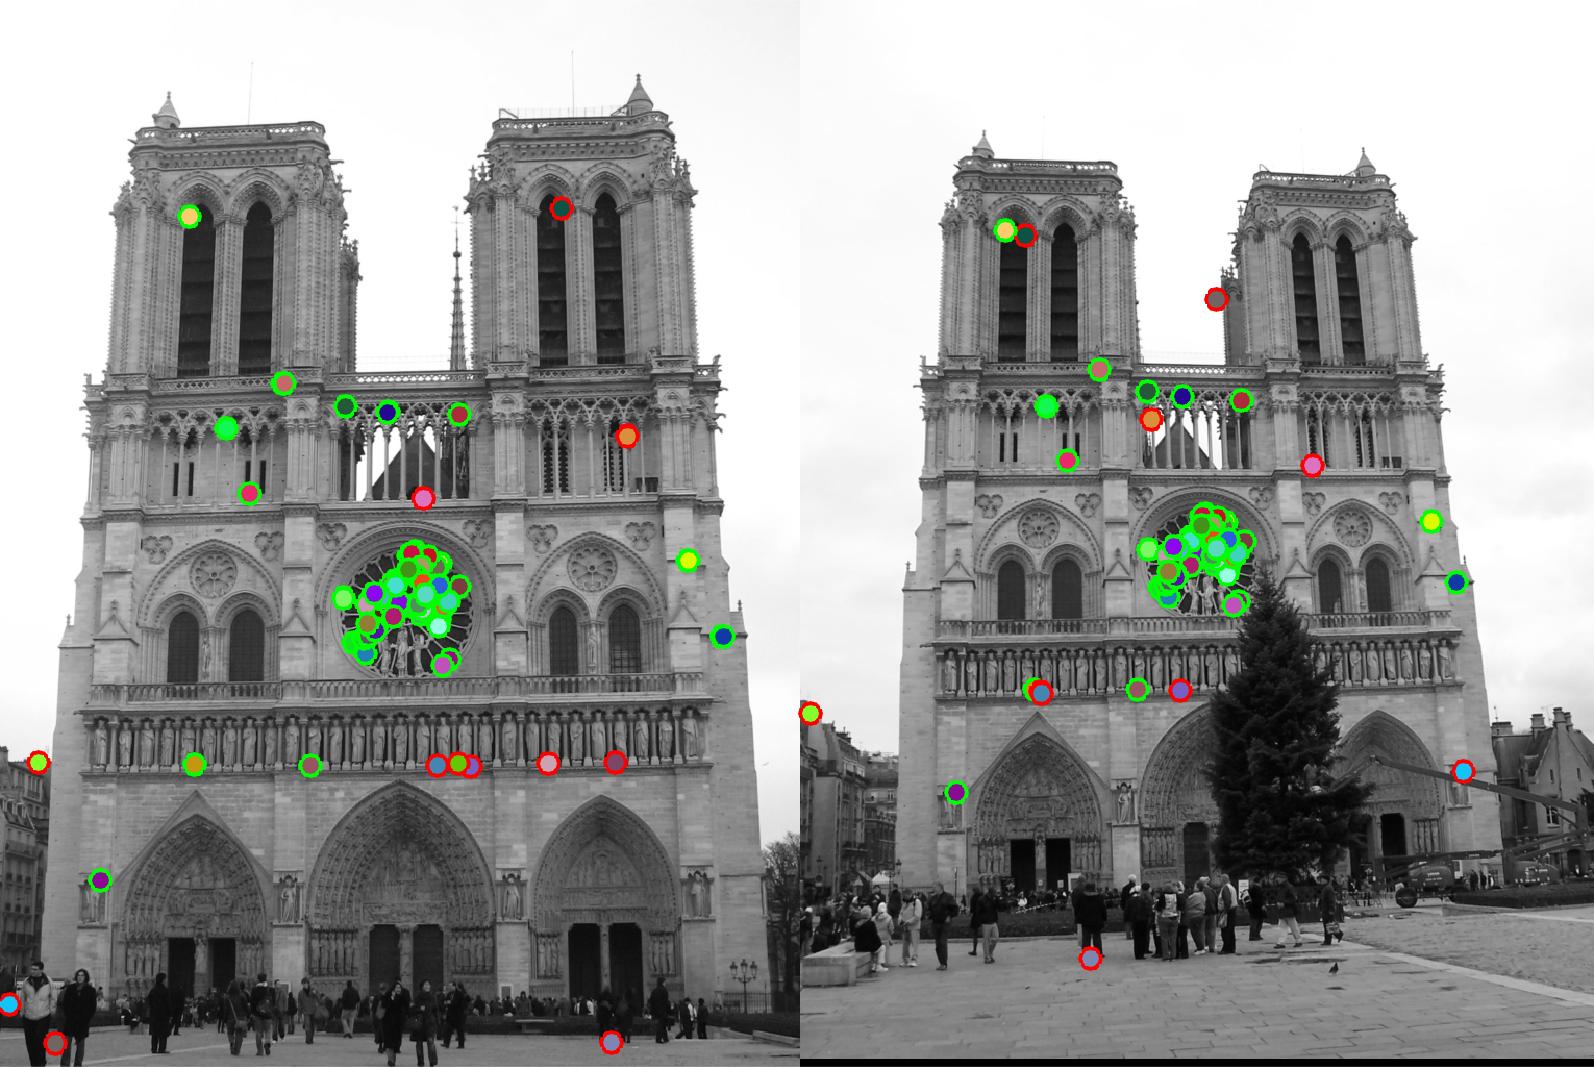
\includegraphics[width=0.7\textwidth]{../code/eval_ND.png}
	\caption{Notre Dame 87\%}
	\label{fig:nd}
\end{figure}

\begin{figure}[h!]
	\centering
	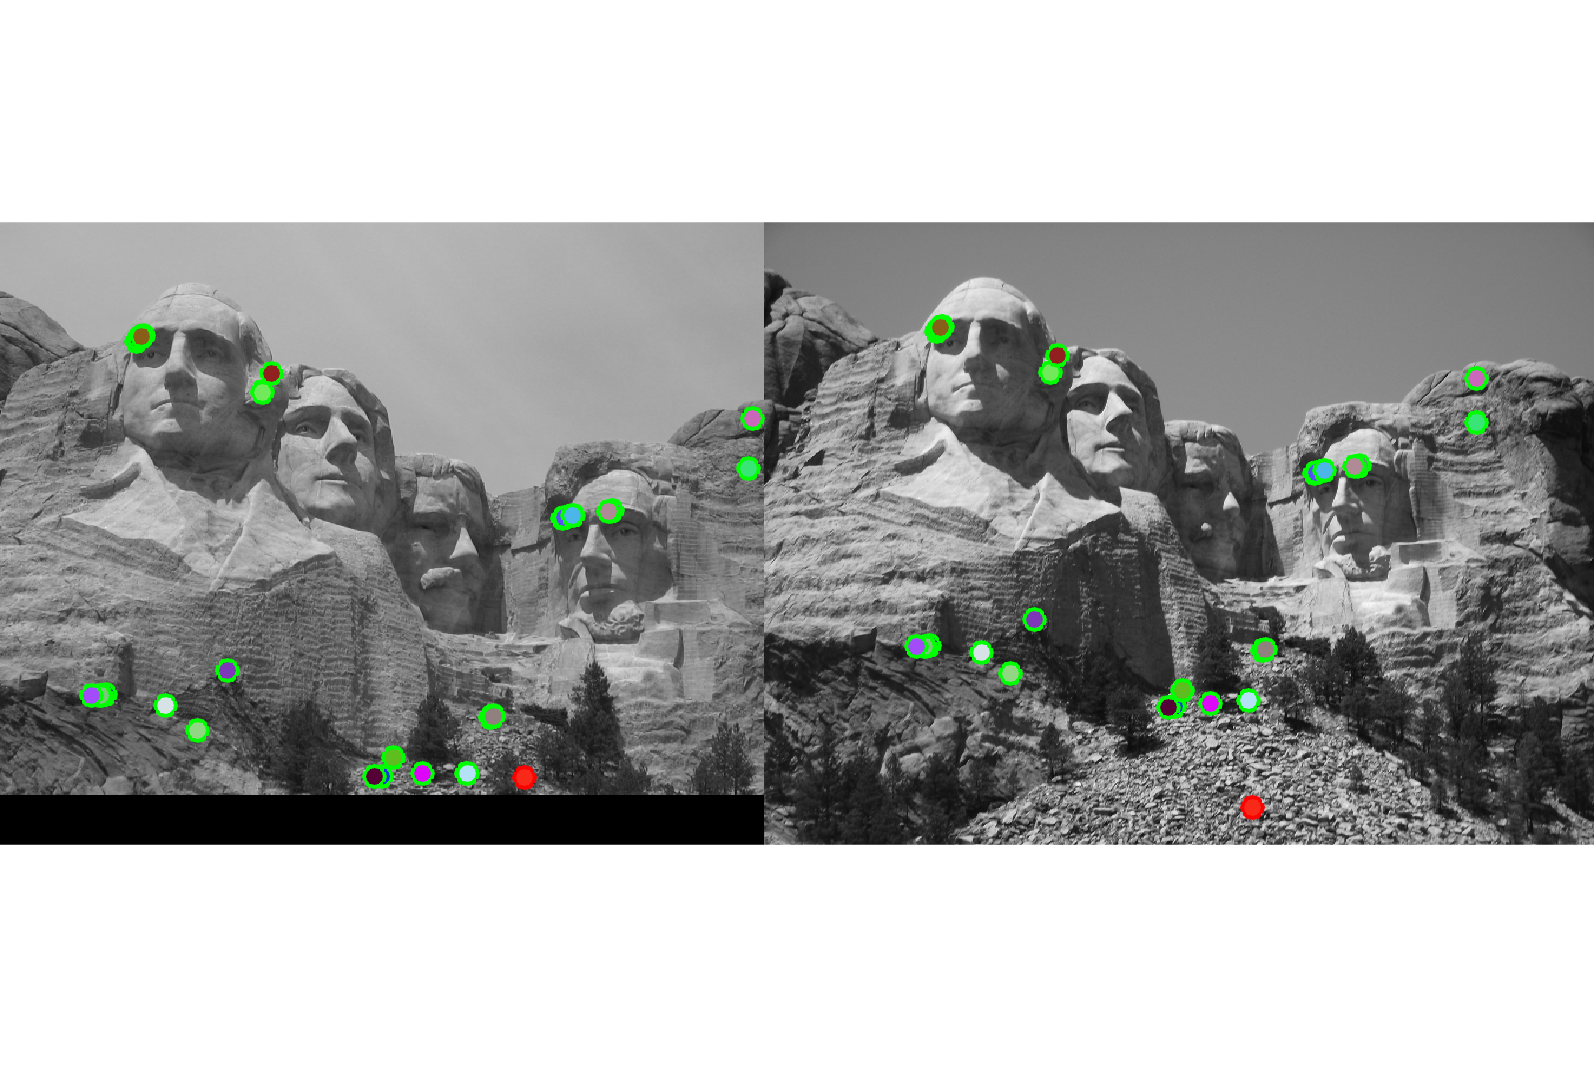
\includegraphics[width=0.7\textwidth]{../code/eval_MR.png}
	\caption{Mount Rushmore 37\%}
	\label{fig:mr}
	\end{figure}
	
\begin{figure}[h!]
	\centering
	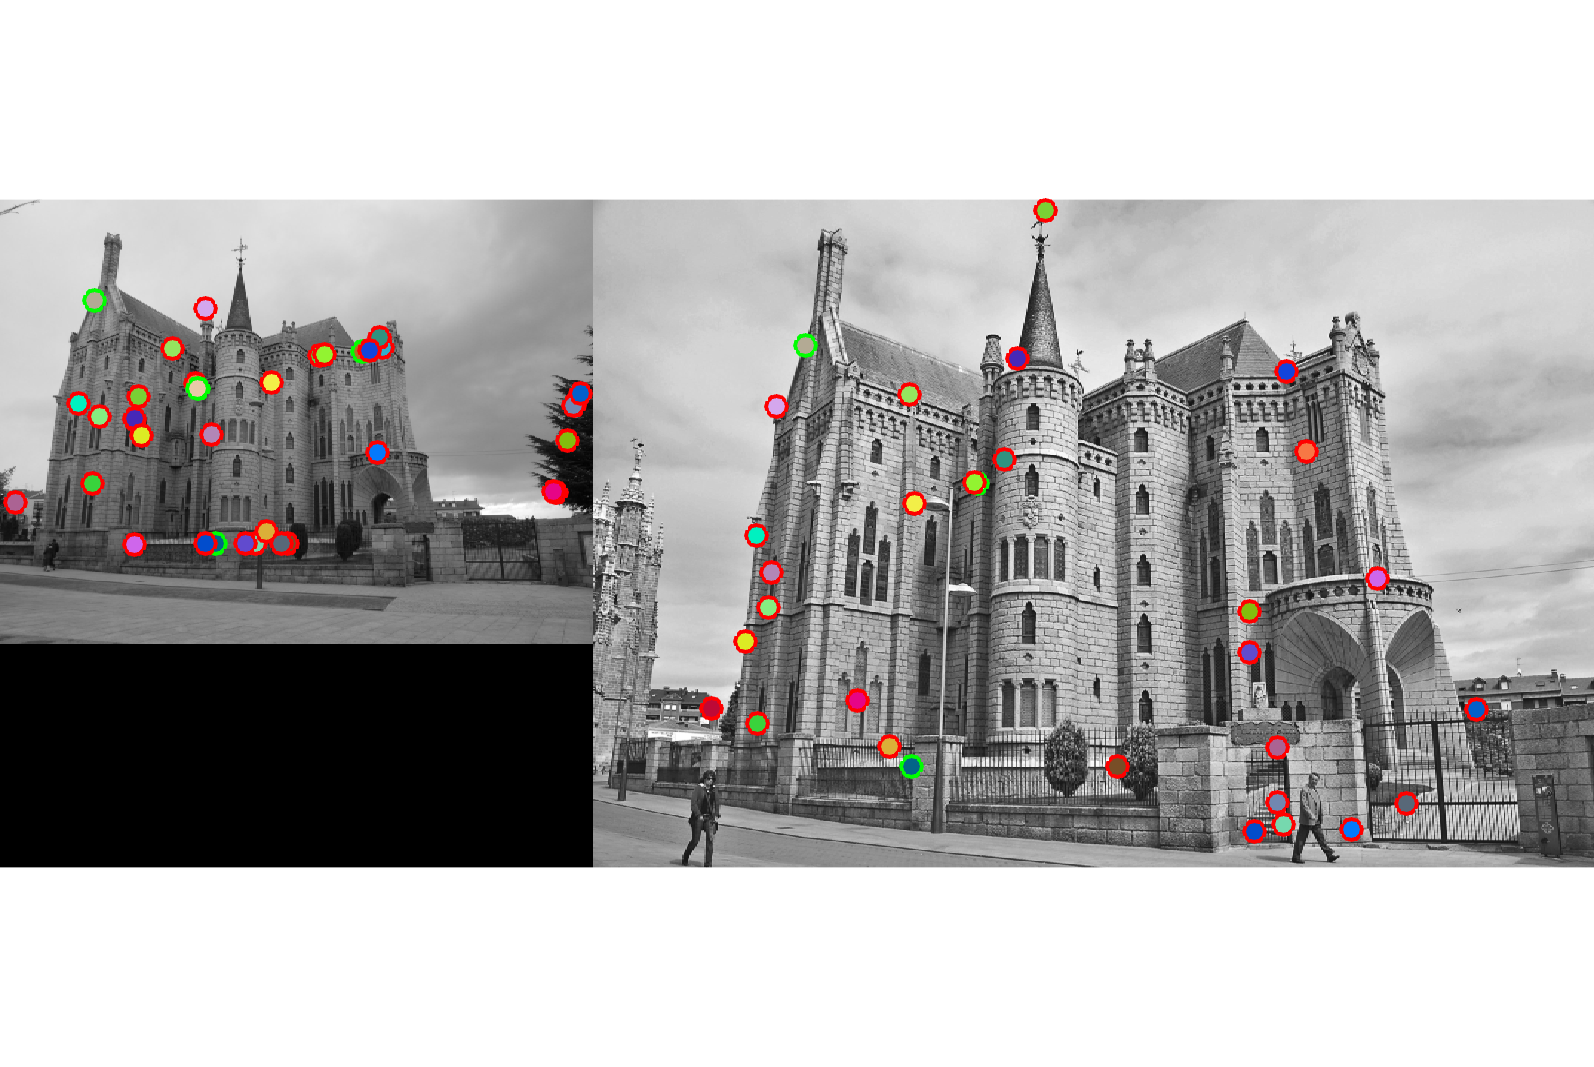
\includegraphics[width=0.7\textwidth]{../code/eval_EG.png}
	\caption{Episcopal Gaudi 5\%}
	\label{fig:eg}
\end{figure}

When trying different parameters such as filter size, sigma and thresholds of feature matching, I realized it influences accuracy of the matching. Time was also measured to make sure the computation does not exceed the time limit. Relevant code shown below. As shown in Figure~\ref{fig:size_comp}, maximum accuracy is obtained at filter size of 4. Time was not influenced by the filter size seemingly because the number of features did not change. Figure~\ref{fig:sigma_comp} compares different amount of sigma while the window size is fixed at 4. The maximum accuracy is therefore attained at sigma of 0.6 and filter size of 4. Time was not influenced by the sigma either.
\begin{lstlisting}[style=Matlab-editor]
size_range = 3:30;
%size_range = 0.1:0.1:1.5;
i = 1;
for s=size_range
	tic;
	% 2) Create feature descriptors at each interest point. Szeliski 4.1.2
	[image1_features] = get_descriptors(image1, x1, y1, descriptor_window_image_width, s);
	[image2_features] = get_descriptors(image2, x2, y2, descriptor_window_image_width, s);
	
	% 3) Match features. Szeliski 4.1.3
	[matches, confidences] = match_features(image1_features, image2_features);
	
	% Evaluate matches
	[~,~,accAll,accMPEND] = evaluate_correspondence(image1, image2, eval_file, scale_factor, ... 
		x1, y1, x2, y2, matches, confidences, ...
		maxPtsEval, visualize, 'eval_ND.png' );
	accs(s) = accAll
	ts(s) = toc
	i = i+1;
end
\end{lstlisting}

\begin{figure}[h!]
	\centering
	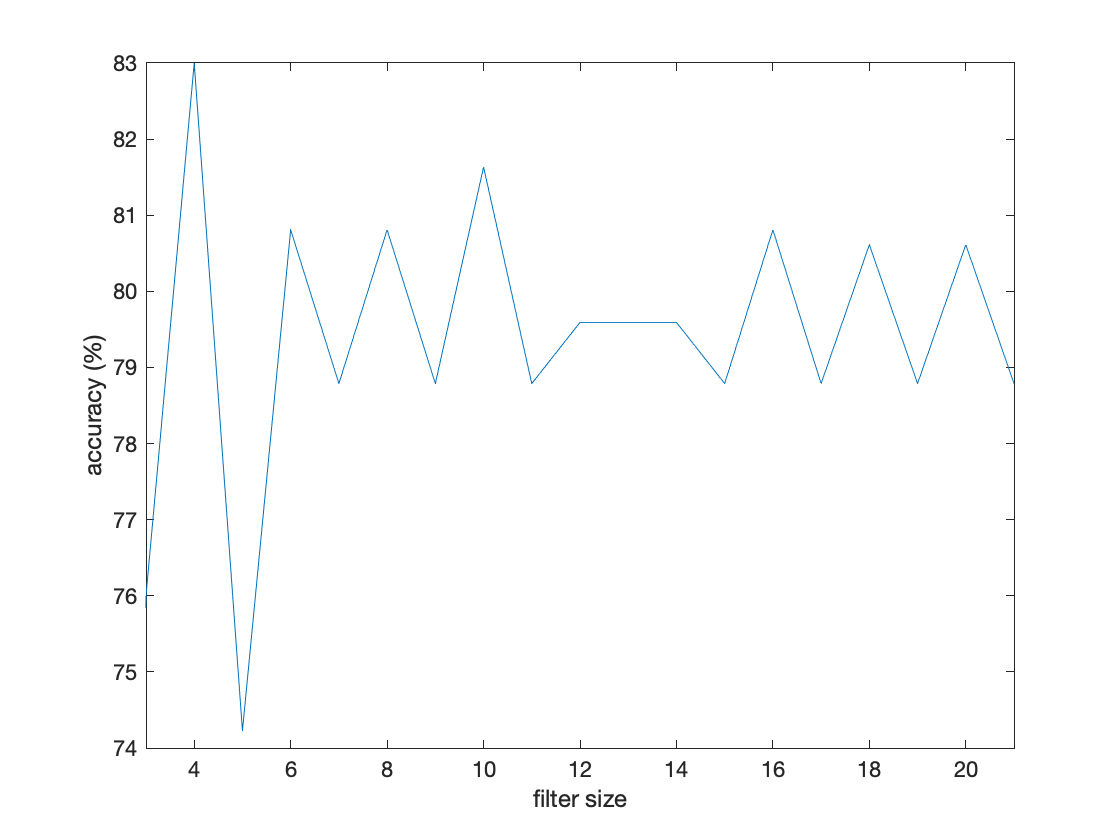
\includegraphics[width=0.45\textwidth]{../code/size_vs_acc.png}
	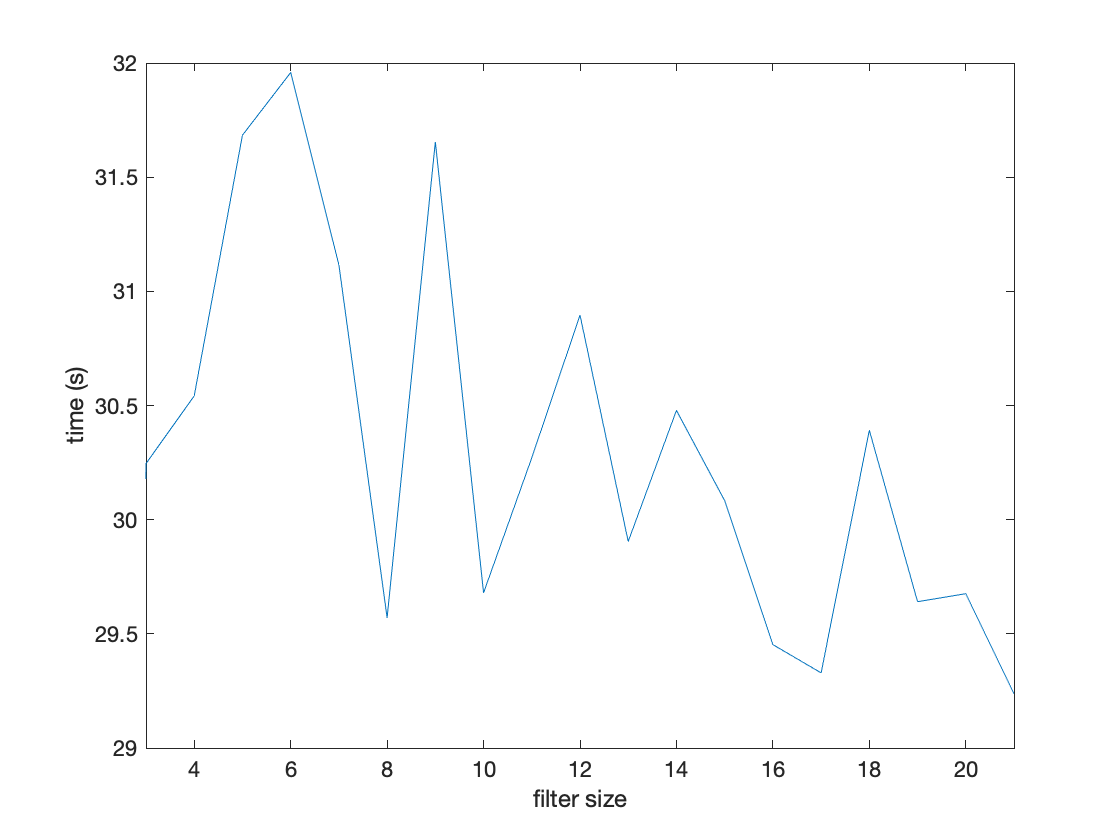
\includegraphics[width=0.45\textwidth]{../code/size_vs_time.png}
	\caption{Size vs Accuracy (left) and Time (right)}
	\label{fig:size_comp}
\end{figure}

\begin{figure}[h!]
	\centering
	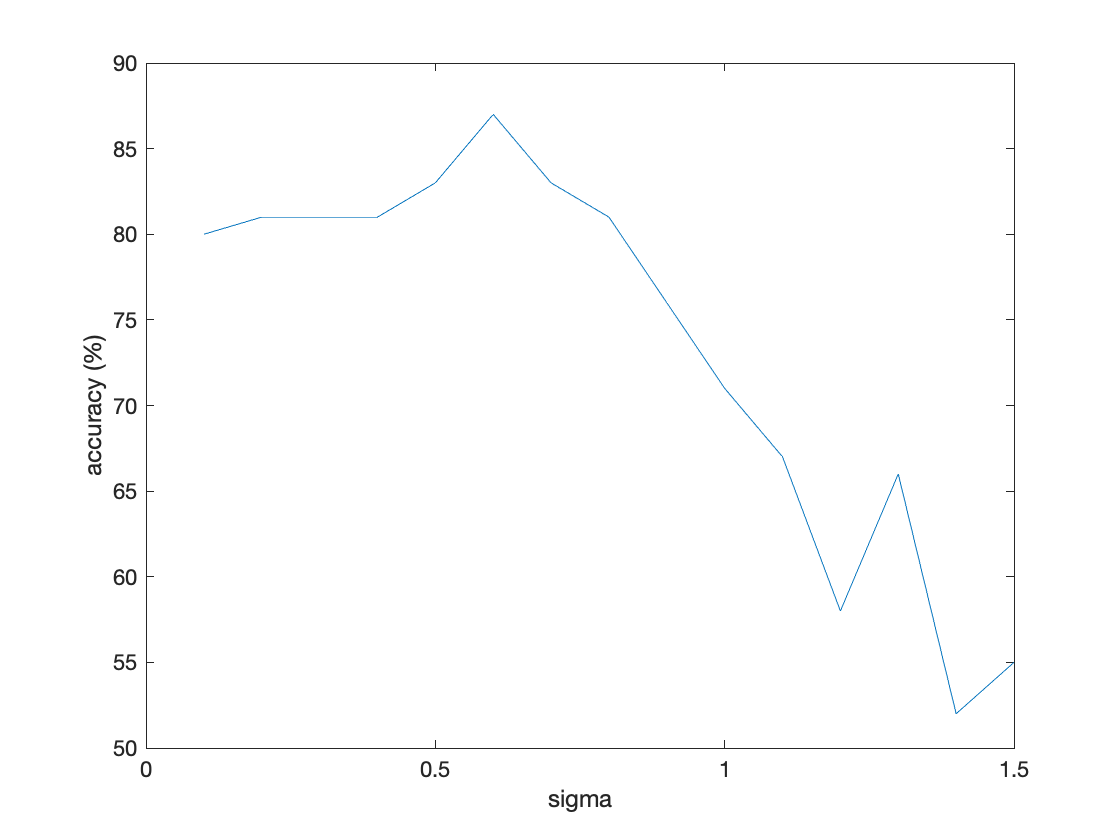
\includegraphics[width=0.45\textwidth]{../code/sigma_vs_acc.png}
	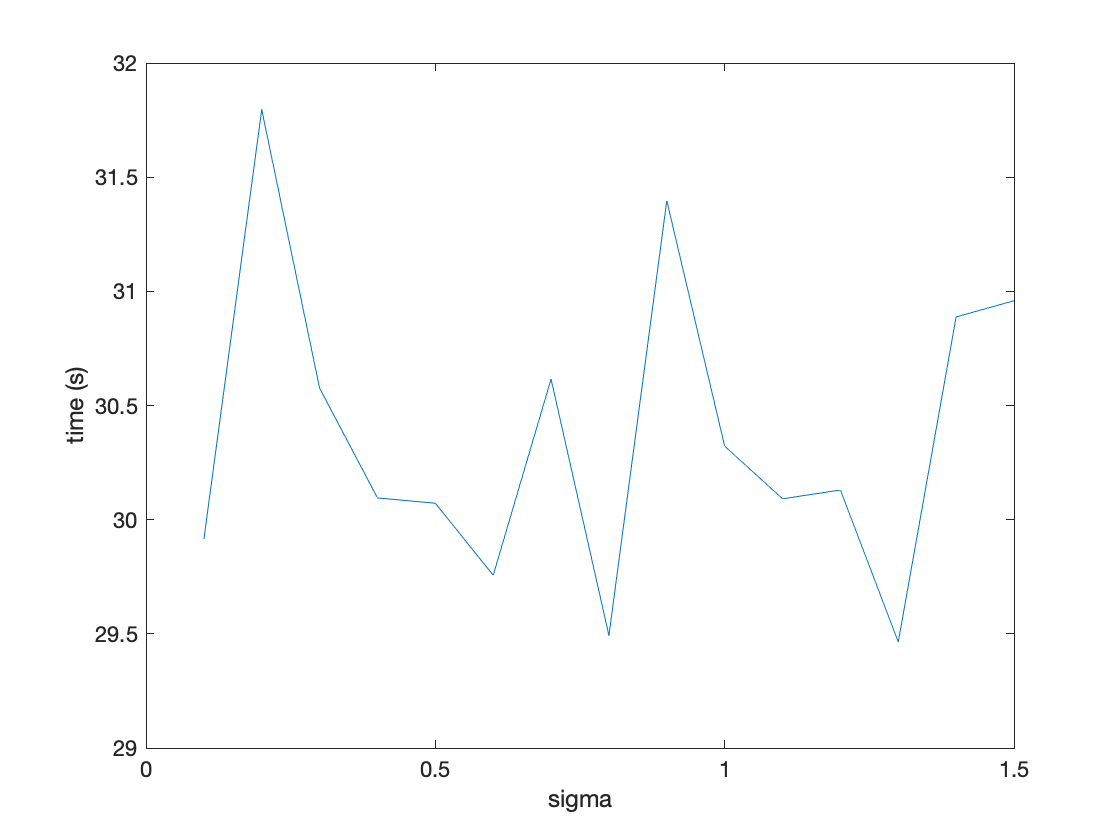
\includegraphics[width=0.45\textwidth]{../code/sigma_vs_time.png}
	\caption{Size vs Accuracy (left) and Time (right)}
	\label{fig:sigma_comp}
\end{figure}

\end{document}
